\subsection{Rank lists fusion}

\subsubsection{Rank list fusion evaluation \label{sec:eval_fusion}}

In this experiment, the goal to understand if fusing rank list can improve performance of the rank list.
The methodology used, is to create $n$ rank lists and fuse them for every $r$ rank lists combinations ($C^n_r$) for the two fusing methods proposed, z-score fusion and regression fusion.

The rank list used are the ones obtained by using the 9 retained rank list methods ($n=9$), see Table~\ref{tab:9rl} in annex.
They represent the best configuration retained for each text representation.
The $r$ value is selected to $4$, since it represents the number of different text representation.
The number of possible fusion combinations is with $n=9$ and $r=4$ is $C^{9}_{4} = 126$.
For this 126 fusions, the 3 metrics: Average Precision (AP), R-Precision (RPrec) and High Precision (HPrec) are computed.

To compare the rank list produced by both the Z-Score fusions and the Regression fusion to the non-fused rank lists, two evaluation strategies are used.
One called \textit{Single-Max} which represent the best metrics for each rank list in the fusion and another one called \textit{Single-Mean} which is represented by the mean of each rank list metrics in the fusion.
For example, if for a fusion the average precision of the 4 rank lists are : $0.5, 0.6, 0.7, 0.8$. Single-mean would have an average precision of $0.65$ and Single-max an average precision of $0.8$.
If the Single-Max evaluation strategy is over-come by a rank list produced by a fusion it means that the resulting rank list give results even better then every individual rank lists used for this fusion, the best case.
For the Single-Mean, if it is over come it means that the obtained rank list have better results than the average results of the rank list, thus when using the system \textit{in the blind} (when the rank list can't be evaluated, with new data for example), fusing is a good approach since it gives stability.

The results of every fusion combinations using the proposed rank list and strategies are graphically presented in Figure~\ref{fig:fusions}.
Statistiques for each metrics and fusion schemes are resumed Tables~\ref{tab:fusion_stats_A_B}/\ref{tab:fusion_stats_B_A}, it contains for each metric, the minimal value (min), the average and the standard deviation (Avg$\pm$Std), the maximal value, the argmin and argmax for the metrics (using ids of the rank list in Table~\ref{tab:9rl} in annex).
A sign test between the two strategies and the two fusion methods is presented in Table~\ref{tab:fusion_sign_test}.

\begin{figure}
  \centering
  \caption{Evaluation of every combination of 4 rank list fusions using Z-Score and Regression}
  \label{fig:fusions}

  \subcaption{Testing on St-Jean A (training St-Jean B, for the Regression fusion)}
  \label{fig:fusion_B_A}
  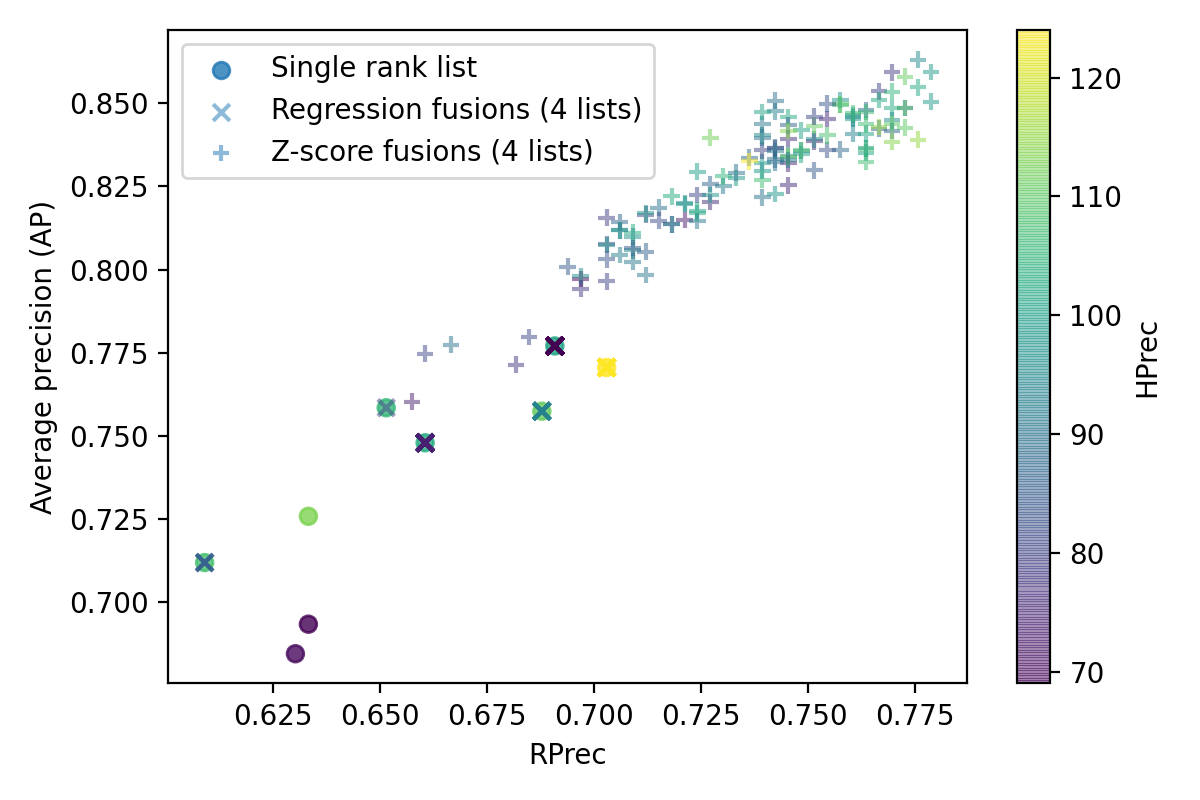
\includegraphics[width=\linewidth]{img/fusion_B_A.png}

  \subcaption{Testing on St-Jean B (training St-Jean A, for the Regression fusion)}
  \label{fig:fusion_A_B}
  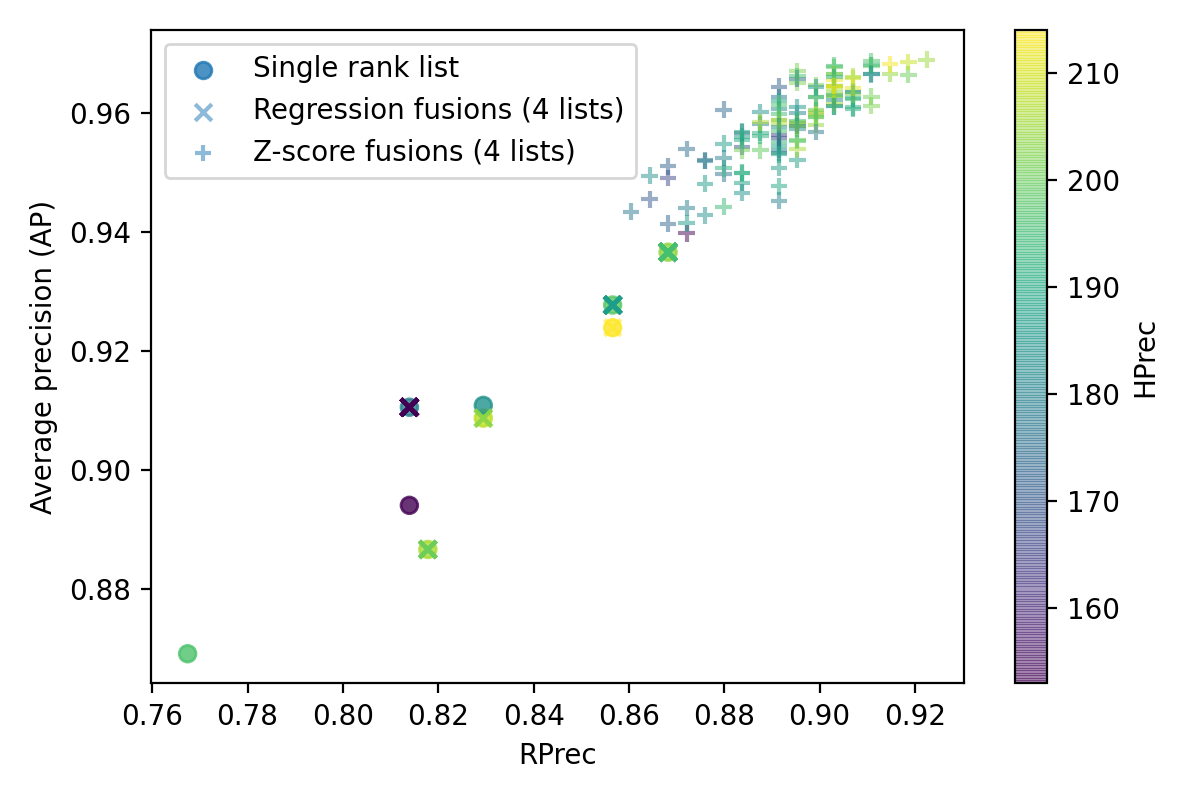
\includegraphics[width=\linewidth]{img/fusion_A_B.png}
\end{figure}

\begin{table}
  \centering
  \caption{Fusion statistics on St-Jean A}
  \label{tab:fusion_stats_A_B}

  \subcaption{Single-Mean}
  \begin{tabular}{l l l l}
    \toprule
    Stats
    & AP
    & RPrec
    & HPrec \\
    \midrule
    Min & $0.704$ & $0.627$ & $42.75$ \\
    Avg$\pm$Std & $0.736\pm0.013$ & $0.656\pm0.012$ & $64.444\pm10.286$ \\
    Max & $0.766$ & $0.686$ & $84.25$ \\
    Argmin & [4,6,7,8] & [4,6,7,8] & [0,1,6,7] \\
    Argmax & [0,2,3,5] & [0,1,2,3] & [2,3,4,8] \\
    \bottomrule
  \end{tabular}

  \subcaption{Single-Max}
  \begin{tabular}{l l l l}
    \toprule
    Stats
    & AP
    & RPrec
    & HPrec \\
    \midrule
    Min & $0.726$ & $0.633$ & $68.0$ \\
    Avg$\pm$Std & $0.769\pm0.009$ & $0.692\pm0.015$ & $88.532\pm9.763$ \\
    Max & $0.777$ & $0.703$ & $99.0$ \\
    Argmin & [4,6,7,8] & [4,6,7,8] & [0,1,6,7] \\
    Argmax & [0,1,2,3] & [0,1,2,3] & [0,1,2,3] \\
    \bottomrule
  \end{tabular}

  \subcaption{Z-Score}
  \begin{tabular}{l l l l}
    \toprule
    Stats
    & AP
    & RPrec
    & HPrec \\
    \midrule
    Min & $0.76$ & $0.658$ & $69.0$ \\
    Avg$\pm$Std & $0.829\pm0.02$ & $0.738\pm0.026$ & $93.833\pm11.108$ \\
    Max & $0.863$ & $0.779$ & $124.0$ \\
    Argmin & [4,5,6,7] & [4,5,6,7] & [0,1,4,5] \\
    Argmax & [0,3,7,8] & [0,3,6,8] & [1,3,6,7] \\
    \bottomrule
  \end{tabular}

  \subcaption{Regression (training St-Jean B)}
  \begin{tabular}{l l l l}
    \toprule
    Stats
    & AP
    & RPrec
    & HPrec \\
    \midrule
    Min & $0.712$ & $0.609$ & $65.0$ \\
    Avg$\pm$Std & $0.764\pm0.016$ & $0.681\pm0.02$ & $72.794\pm12.111$ \\
    Max & $0.777$ & $0.703$ & $99.0$ \\
    Argmin & [4,5,6,7] & [4,5,6,7] & [0,1,2,3] \\
    Argmax & [0,1,2,3] & [2,3,4,5] & [2,3,4,5] \\
    \bottomrule
  \end{tabular}
\end{table}

\begin{table}
  \centering
  \caption{Fusion statistics on St-Jean B}
  \label{tab:fusion_stats_B_A}

  \subcaption{Single-Mean}
  \begin{tabular}{l l l l}
    \toprule
    Stats
    & AP
    & RPrec
    & HPrec \\
    \midrule
    Min          & $0.89$         & $0.80$         & $122.25$      \\
    Avg$\pm$Std & $0.90\pm0.008$ & $0.83\pm0.011$ & $148.11\pm11$ \\
    Max          & $0.92$         & $0.85$         & $172$         \\
    Argmin       & [3,4,7,8]   & [1,3,7,8]   & [1,6,7,8]  \\
    Argmax       & [0,2,5,6]   & [0,2,5,6]   & [0,3,4,5]  \\
    \bottomrule
  \end{tabular}

  \subcaption{Single-Max}
  \begin{tabular}{l l l l}
    \toprule
    Stats
    & AP
    & RPrec
    & HPrec \\
    \midrule
    Min          & $0.91$         & $0.82$         & $153.25$      \\
    Avg$\pm$Std & $0.93\pm0.008$ & $0.86\pm0.012$ & $174.8\pm7$ \\
    Max          & $0.93$         & $0.87$         & $182$         \\
    Argmin       & [3,4,7,8]   & [1,3,7,8]   & [1,6,7,8]  \\
    Argmax       & [0,1,2,3]   & [0,1,2,3]   & [0,1,2,5]  \\
    \bottomrule
  \end{tabular}

  \subcaption{Z-Score}
  \begin{tabular}{l l l l}
    \toprule
    Stats
    & AP
    & RPrec
    & HPrec \\
    \midrule
    Min          & $0.94$         & $0.86$         & $153$      \\
    Avg$\pm$Std & $0.96\pm0.006$ & $0.89\pm0.012$ & $191.3\pm12$ \\
    Max          & $0.97$         & $0.82$         & $214$         \\
    Argmin       & [1,2,3,8]   & [2,3,4,8]   & [1,2,3,8]  \\
    Argmax       & [1,2,5,6]   & [1,2,5,6]   & [2,3,5,7]  \\
    \bottomrule
  \end{tabular}

  \subcaption{Regression (training St-Jean A)}
  \begin{tabular}{l l l l}
    \toprule
    Stats
    & AP
    & RPrec
    & HPrec \\
    \midrule
    Min          & $0.88$         & $0.81$         & $124$      \\
    Avg$\pm$Std & $0.92\pm0.015$ & $0.85\pm0.024$ & $152.9\pm18$ \\
    Max          & $0.94$         & $0.87$         & $182$         \\
    Argmin       & [3,4,5,6]   & [1,2,3,4]   & [1,2,3,4]  \\
    Argmax       & [0,1,2,3]   & [0,1,2,3]   & [5,6,7,8]  \\
    \bottomrule
  \end{tabular}
\end{table}

\begin{table*}
  \centering
  \caption{Rank list fusion sign test. \textit{The star (*) indicate a Binomial test p-value smaller than 5\%}}
  \label{tab:fusion_sign_test}

  \subcaption{Testing St-Jean A (training St-Jean B, for the Regression fusion)}
  \label{tab:fusion_A_B}
  \begin{tabular}{l c c c c}
    \toprule
    Metric
    & Z-Score/T/Single-Mean
    & Z-Score/T/Single-Max
    & Regression/T/Single-Mean
    & Regression/T/Single-Max\\
    \midrule
    AP    & *126/0/0 & *126/0/0  & *108/0/18 & 0/81/45* \\
    RPrec & *126/0/0 & *125/1/0  & *92/4/30  & 0/78/48* \\
    HPrec & *126/0/0 & *111/0/14 & *79/1/46  & 0/14/112*\\
    \bottomrule
  \end{tabular}

  \subcaption{Testing St-Jean B (training St-Jean A, for the Regression fusion)}
  \label{tab:fusion_B_A}
  \begin{tabular}{l c c c c}
    \toprule
    Metric
    & Z-Score/T/Single-Mean
    & Z-Score/T/Single-Max
    & Regression/T/Single-Mean
    & Regression/T/Single-Max \\
    \midrule
    AP    & *126/0/0 & *124/0/2 & *120/0/6  & 0/85/41* \\
    RPrec & *126/0/0 & *119/2/5 & *114/0/12 & 0/76/50* \\
    HPrec & *124/0/2 & *73/3/45 & *92/0/34  & 0/25/101*\\
    \bottomrule
  \end{tabular}

\end{table*}

Using these distance metrics on St-jean, the sign test tends to indicate that the fusion increase the overall quality of the rank list.
The three evaluations metrics are high correlated (especially average precision and R-Precision), only the average precision will be explored in depth.
The Z-Score fusion, produce for every metrics better results than both Single-Mean and Single-Max, the average precision is increase in average by $\sim 10$\% compared to the average of the average precision (Single-Mean) of the rank list used, and by ~6\% in average when considering the maximal average precision (Single-Max).
In the other hand, the Regression fusion, have an average increase of $\sim 3$\% in average precision for the Single-Mean and have a decrease of ~1\% when comparing to the Single-Max.
A general observation of the Tables, show that the HPrec tends to be the least easy metric to increase when using the fusion.
The results of fusing multiple rank lists when using regression fusion strategy tends to indicate that the resulting rank list has in average the same quality as the best rank list used for the fusion with some slight decreases.
This can be further confirmed by looking at Table~\ref{tab:fusion_B_A}, which shows in the column Regression/T/Single-Max more ties than the average and in Figure~\ref{fig:fusions} where most Regression score and and Single rank list score overlap.
No particular set of rank list tends to give the best results in every case when fusing with the two strategies, every rank list is present in the argmax, but with the Z-Score fusion, the best results seem to be obtained with rank lists using different text representations.
The Z-score fusion give the best results overall.

\subsubsection{Fusion veto}

In this experiment, the goal is to understand if the veto method can improve the average precision on the fused rank lists using the regression fusion method.

To do so, the St-Jean retained rank list are used (ref. Table~\ref{tab:9rl_results_st_jean} in annex).
The fusion scheme is learnt on first St-Jean A and trained on St-Jean B (ref. Section~\ref{sec:regression_fusion}), then the inverse.
After computing the probabilities for each link in each rank list on the testing set, the probabilities under the threshold are set according to each proposed veto strategy (set to $0$, $-1$, $-n$, $-\infty$).
The threshold is analysed for the vales between $0.01$ and $0.50$, with a step of $0.01$.
After a threshold of $0.50$, the veto shouldn't be applied since it corresponds to the probability of being a false link is smaller than the probability of being a true link.
The fusion of the rank list is normally computed with the average of the probabilities.
When computing the average of the probabilities when containing $-\infty$ always yield a $-\infty$ probability.
To understand if the veto improve the results, the difference between the average precision of the rank list obtained by fusing with the veto strategy and the average precision of the rank list without the veto is computed.

The average precision difference over the threshold value is visually presented in Figure~\ref{fig:veto}, and the best configurations found are summarized in Table~\ref{tab:veto}.

\begin{figure}
  \caption{Veto strategies evaluations on St-Jean A and B depending on the threshold}
  \label{fig:veto}
  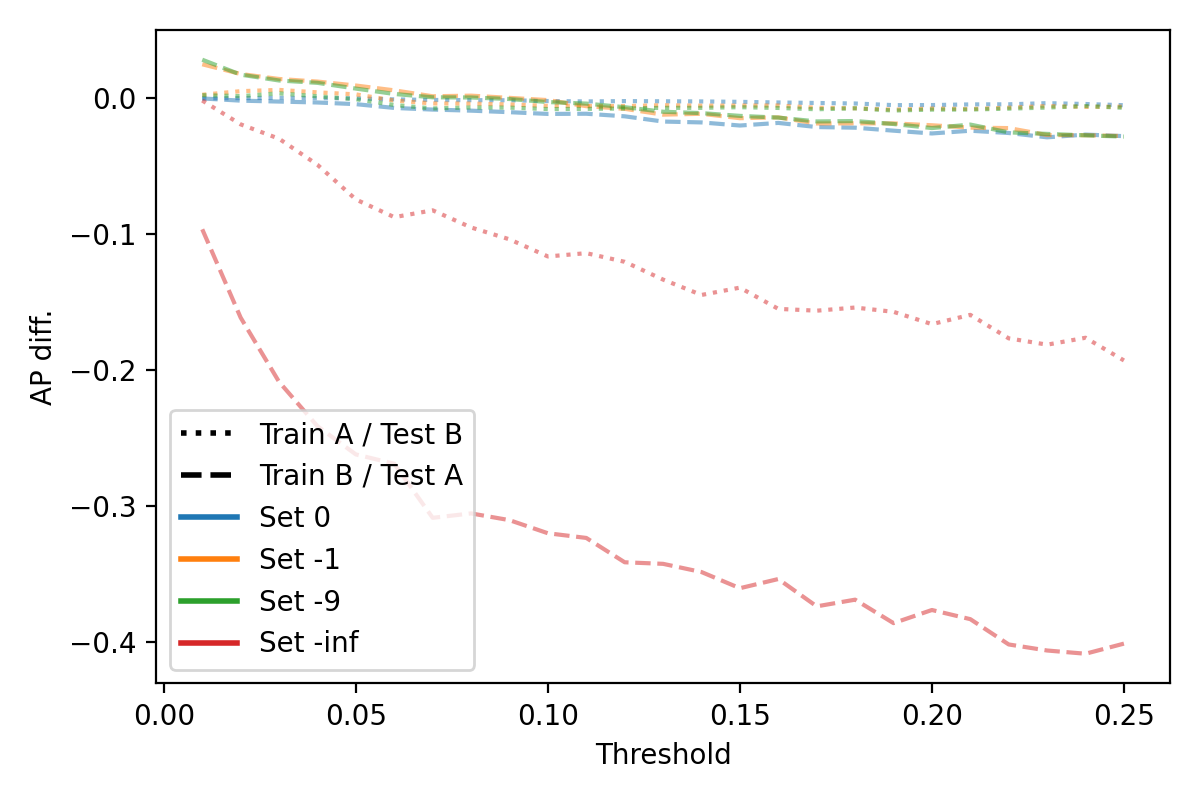
\includegraphics[width=\linewidth]{img/veto.png}
\end{figure}

\begin{table}
  \centering
  \caption{Maximal gain on the average precision using the veto / Argmax}
  \label{tab:veto}
  \begin{tabular}{l r r}
    \toprule
                   & Train A / Test B & Train B / Test A \\
    \midrule
    Set to $0$     & 0.000/0.03       & 0.000/0.01       \\
    Set to $-1$    & 0.006/0.03       & 0.025/0.01       \\
    Set to $-n$    & 0.004/0.03       & 0.028/0.01       \\
    Set to $-\inf$ & -0.002/0.01      & -0.096/0.01      \\
    \bottomrule
  \end{tabular}
\end{table}

The overall the veto strategy seem to be a bad option.
The best result obtained is only an increase of 0.028 in average precision, with a tiny threshold (the closest to a non threshold approach) which may indicate an increase due to random factors.
Using the infinity strategy only give worse results.
